
%%%%%%%%%%%%%%%%%%%%%%%%%%%%%%%%%%%%%%%%%%%%%%%%%%%%%%%%%%%%%%%%%%%%%%%%%%%%%%%%%%%%%%%
%%%%%%%%%%%%%%%%%%%%%%%%%%%%%%%%%%%%%%%%%%%%%%%%%%%%%%%%%%%%%%%%%%%%%%%%%%%%%%%%%%%%%%%
% 
% This top part of the document is called the 'preamble'.  Modify it with caution!
%
% The real document starts below where it says 'The main document starts here'.

\documentclass[12pt]{article}

\usepackage{amssymb,amsmath,amsthm}
\usepackage[top=1in, bottom=1in, left=1.25in, right=1.25in]{geometry}
\usepackage{fancyhdr}
\usepackage{enumerate}
\usepackage{listings}
\usepackage{graphicx}
\usepackage{float}
% Comment the following line to use TeX's default font of Computer Modern.

\usepackage{times,txfonts}



\makeatletter
\renewcommand*\env@matrix[1][*\c@MaxMatrixCols c]{%
  \hskip -\arraycolsep
  \let\@ifnextchar\new@ifnextchar
  \array{#1}}
\makeatother

\newtheoremstyle{homework}% name of the style to be used
  {18pt}% measure of space to leave above the theorem. E.g.: 3pt
  {12pt}% measure of space to leave below the theorem. E.g.: 3pt
  {}% name of font to use in the body of the theorem
  {}% measure of space to indent
  {\bfseries}% name of head font
  {:}% punctuation between head and body
  {2ex}% space after theorem head; " " = normal interword space
  {}% Manually specify head
\theoremstyle{homework} 

% Set up an Exercise environment and a Solution label.
\newtheorem*{exercisecore}{Exercise \@currentlabel}
\newenvironment{exercise}[1]
{\def\@currentlabel{#1}\exercisecore}
{\endexercisecore}

\newcommand{\localhead}[1]{\par\smallskip\noindent\textbf{#1}\nobreak\\}%
\newcommand\solution{\localhead{Solution:}}

%%%%%%%%%%%%%%%%%%%%%%%%%%%%%%%%%%%%%%%%%%%%%%%%%%%%%%%%%%%%%%%%%%%%%%%%
%
% Stuff for getting the name/document date/title across the header
\makeatletter
\RequirePackage{fancyhdr}
\pagestyle{fancy}
\fancyfoot[C]{\ifnum \value{page} > 1\relax\thepage\fi}
\fancyhead[L]{\ifx\@doclabel\@empty\else\@doclabel\fi}
\fancyhead[C]{\ifx\@docdate\@empty\else\@docdate\fi}
\fancyhead[R]{\ifx\@docauthor\@empty\else\@docauthor\fi}
\headheight 15pt

\def\doclabel#1{\gdef\@doclabel{#1}}
\doclabel{Use {\tt\textbackslash doclabel\{MY LABEL\}}.}
\def\docdate#1{\gdef\@docdate{#1}}
\docdate{Use {\tt\textbackslash docdate\{MY DATE\}}.}
\def\docauthor#1{\gdef\@docauthor{#1}}
\docauthor{Use {\tt\textbackslash docauthor\{MY NAME\}}.}
\makeatother

% Shortcuts for blackboard bold number sets (reals, integers, etc.)
\newcommand{\Reals}{\ensuremath{\mathbb R}}
\newcommand{\Nats}{\ensuremath{\mathbb N}}
\newcommand{\Ints}{\ensuremath{\mathbb Z}}
\newcommand{\Rats}{\ensuremath{\mathbb Q}}
\newcommand{\Cplx}{\ensuremath{\mathbb C}}
%% Some equivalents that some people may prefer.
\let\RR\Reals
\let\NN\Nats
\let\II\Ints
\let\CC\Cplx

%%%%%%%%%%%%%%%%%%%%%%%%%%%%%%%%%%%%%%%%%%%%%%%%%%%%%%%%%%%%%%%%%%%%%%%%%%%%%%%%%%%%%%%
%%%%%%%%%%%%%%%%%%%%%%%%%%%%%%%%%%%%%%%%%%%%%%%%%%%%%%%%%%%%%%%%%%%%%%%%%%%%%%%%%%%%%%%
% 
% The main document start here.

% The following commands set up the material that appears in the header.
\doclabel{STAT 402: Homework 11}
\docauthor{Stefano Fochesatto}
\docdate{\today}


%\textbf{Code:}
%\begin{center}
 %   \lstinputlisting{r1.txt}
%\end{center}

\begin{document}

\begin{exercise}{1} We will slowly go through a distance analysis by hand:\\
  Suppose we walked a single transect that was 500 m long and counted every squirrel we see. Our truncation distance is 30 m and the transect was randomly positioned in a region of 1 square Kilometer.
  We obtained the following distances (in meters) to the squirrels sighted, perpendicular distance to the transect (call these Dists from now on):\\
  17.9, 0.3, 7.3, 16.0, 3.6, 33.7, 19.4, 11.0, 1.3, 2.6, 0.8, 25.9, 3.7, 1.1, 4.1, \\
  1.3, 0.0, 8.0, 21.0, 13.7, 6.7, 14.4, 9.4, 10.7, 2.0, 8.3, 7.6, 6.5, 3.1, 12.3

  or, as R data:\\
  c(17.9, 0.3, 7.3, 16, 3.6, 33.7, 19.4, 11, 1.3, 2.6, 0.8, 25.9, 3.7, 1.1, 4.1,\\
  1.3, 0, 8, 21, 13.7, 6.7, 14.4, 9.4, 10.7, 2, 8.3, 7.6, 6.5, 3.1, 12.3)
  
  \begin{enumerate}
    \item[a.] Make a histogram plot showing the proportion in 0 to 5m, 5 to 10m, 10 to 20m, etc. Of the models: Uniform (flat), half-normal and (negative) exponential, which seems to be a better fit?\\
    \solution Looking at the histogram I would suggests that negative exponential looks to be the best fit, but it might be worthwhile to experiment with the half-normal as well.
    \begin{figure}[H]
      \begin{center}
      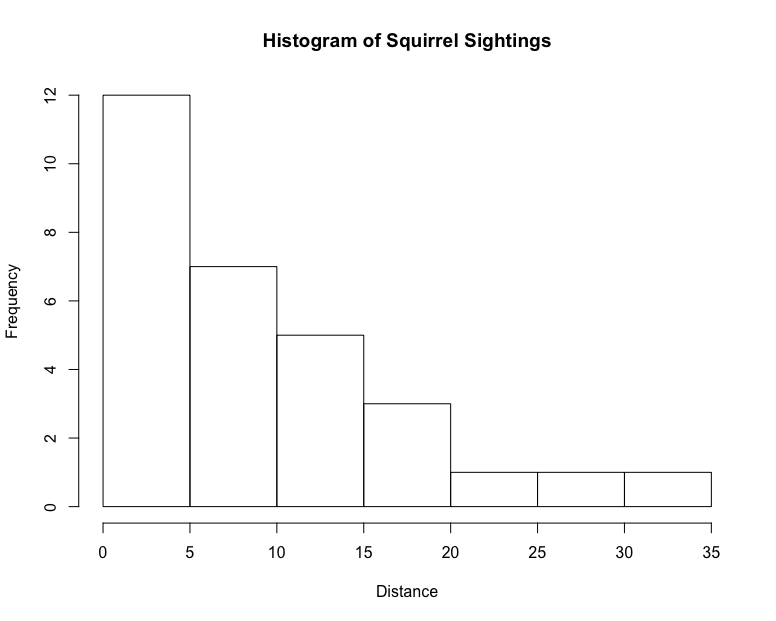
\includegraphics[width = .9\textwidth]{Rplot.png}
      \end{center}
    \end{figure}  

    \vspace{.15in}



    \item[b.]  Let’s try the exponential model. It has the probability function $ f(x) = \dfrac{1}{b}e^{\dfrac{-x}{b}}$, where $b$ is the parameter we need to estimate. In this case, 
    the maximum likelihood estimate of $b$ is just the mean of the $x$ values. Compute the fitted density function (that is, plug the estimated $b$ into the probability function).\\
    \solution Computing the mean of the distances we get, $b =  9.123$. Therefore our probability function looks like, 
    \begin{equation*}
      p(x) = \dfrac{1}{9.123}e^{\dfrac{-x}{9.123}}
    \end{equation*}

    \vspace{.15in}


    \item[c.] Now plug each distance into the fitted probability function to get 30 probability values. 
    Multiply these all together. This is the likelihood. The AIC is then $-2ln(likelihood) + 2(number of parameters)$. 
    In this case, the number of parameters is 1 (only b). What is the AIC of this model?\\
    \solution Computing the likelihood and AIC in r we get an AIC of 194.6501, \\
    \textbf{Code:}
    \begin{center}
       \lstinputlisting{r1.txt}
    \end{center}

    \vspace{.15in}

    \item[d.]  Finally, compute $f(0)$, which you get by plugging zero into the density function you obtained in part (b). 
    Plug this value into the line transect density formula to estimate the density of squirrels per square meter. 
    Convert this to an estimate of the density per square Kilometer.\\
    \solution Recall that the line transect density estimator formula is given by,
    \begin{equation*}
      \hat{\lambda} = \frac{n\hat{f}(0)}{2L}.
    \end{equation*}
    Computing the estimator in r we get the following, \\
    \textbf{Code:}
    \begin{center}
       \lstinputlisting{r2.txt}
    \end{center}

  \end{enumerate}
\end{exercise}


\begin{exercise}{2} Now repeat the above analysis for the case where you use a half-normal probability
  function.\\

  \begin{enumerate}
    \item[a.] In this case the formula for the probability function is $f(x) = \frac{\sqrt{2}}{\sqrt{\pi}\sigma} e^{-\frac{x^2}{2\sigma^2}}$ .  
    The maximum likelihood estimator of $\sigma$ is rather simple: first, square all the distances, then average them, 
    then take the square root of this number. What is the detection function (after you plug in your estimated $\sigma$)?\\
    \solution Computing the maximum likelihood estimator of $\sigma$ in r we get, $\sigma = 12.2075$. So our half-normal probability function 
    comes out to be, 
    \begin{equation*}
      f(x) =  \dfrac{\sqrt{2}}{\sqrt{\pi}(12.2075)} e^{-\dfrac{x^2}{2(12.2075)^2}}
    \end{equation*}
    \vspace{.15in}


    \item[b.] This was a maximum likelihood estimator of $\sigma$. In general, how do you get maximum likelihood estimators?  (i.e. what **IS** a maximum likelihood estimator)?\\
    \solution As we described in the previous homework likelihood is used to describe the joint probability of achieving our sampled data given 
    certain model parameters. The maximum likelihood estimator is the model parameters which maximizes that joint probability. In general deriving the estimator 
    involves forming the likelihood function and then taking the derivative with respect to the model parameters and solving for when it equals zero, like any other optimization problem.
    Note that since the likelihood function is often a very large product (depending on size of data), usually we compute the log-likelihood function in order to avoid overflow errors. 
    \vspace{.15in}


    \item[c. ] Next, plug each distance into the probability function to get 30 probabilities. Multiply
    these together to get the likelihood. Then compute the AIC. How does it  compare to the AIC for the exponential model? Which model fits best?\\
    \solution  Computing the AIC in r we get a value of 195.6705, recall that the exponential model achieved 194.6501 which is slightly better. \\
    \textbf{Code:}
    \begin{center}
       \lstinputlisting{r3.txt}
    \end{center}
    
    \vspace{.15in}



    \item[d.] Finally, compute $f(0)$, then compute the density of squirrels under the half-normal model.\\
    \solution Computing the density in r we get that the half-normal model gives us 1960.806 squirrels per square kilometer, \\
    \textbf{Code:}
    \begin{center}
       \lstinputlisting{r4.txt}
    \end{center}
  
  \end{enumerate}

\end{exercise}
\vspace{1in}


\begin{exercise}{3} There is a good reason for truncation. Suppose you were using the exponential model, but the last squirrel you saw wasn’t at 
  12.3 meters: due to an amazing circumstance you managed to see a squirrel at a distance of 180 m, across a small clearing. How much 
  does your estimated density change when you use this new observation? ( You don't have to calculate the AIC, but the effect on the 
  AIC is very severe, also, which puts the entire model in doubt.)\\
  \solution Recomputing the density with a new last encounter and the exponential model we get a value of 2038.967 squirrels per kilometer. This is a dramatically 
  different from the previous calculation. \\
  \textbf{Code:}
  \begin{center}
     \lstinputlisting{r5.txt}
  \end{center}
\end{exercise}
\vspace{1in}



\begin{exercise}{4} I have attached two papers. The first paper (Harbor Porpoises) discusses a line 
  transect survey. Give a brief description of the survey. In particular, why did they stratify the study?\\
  \solution The goal of the survey was to record the distribution, abundance, and trends of Harbor Porpoise in the Glacier 
  Bay National Park and the Icy Strait. From 1991 to 1993 line transect surveys were conducted three times a year to record baseline abundance and distribution patterns as well as 
  population estimates for the total number of Harbor Porpoises. Between 94 to 05 the surveys were continued, Harbor Porpoise presence data was collected(not via line-transect survey) 
  as a by product of a 12 year killer whale survey. This data showed fewer Porpoise encounters, however the study cites this as being likely due to poorer data(no effort data, and differences in methodology.)
  As a result, in order to model the porpoise population 4 years of line transect surveys were conducted with a similar methodology to the early 90's surveys. 
  The region of interest was divided into 5 stratum, and when a sighting was made sighting angle, radar distance, species, counts, and direction of travel were recorded. Search effort was recorded by 
  transect length, weather conditions, visibility index, and observer position. The stratum were decided because previous studies identified that there is plenty of porpoise movement inside of these 'sub regions'
  but not outside, and by stratifying we can take advantage of this behavior to reduce our variance. 
  
\end{exercise}
\vspace{1in}


\begin{exercise}{5} The other paper discusses a study of birds. In this case the authors were worried that one of the main assumptions of line 
  transect studies was violated. What assumption was that? How did they deal with this problem?\\
  \solution The second paper is similar to the first in the sense that the survey was conducted using line transect sampling. The subject of the survey was 
  Murrelets in Glacier Bay National Park. The authors of the survey were very concerned with the assumption of 100 
  percent detection near the center line of the transect, since murrelets are 'small, cryptic, and highly mobile'. To relax this assumption an extra term was added to 
  the density estimator to adjust the detection function(in the paper it is referred to as $P_c$).

\end{exercise}
\vspace{1in}


\begin{exercise}{6} Suppose we wish to monitor changes in the bird population in a 3 square-Kilometer park, over several years. 
  We also would like to get a good estimate of the total population. Our options are:\\
  * Randomly place 10 point transects. Return to the same transects each year.\\
  * Randomly place 10 point transects. Each year re-randomize the locations.\\
  * Randomly place 5 point transects where we will return to each year, and each year place an additional 5 that are just sampled one year.\\
  \begin{enumerate}
    \item[a.] What are the pros and cons of each sampling plan? Which would you recommend?\\
    \solution By selecting the same point transects every year we are allowing more bias to get get a better picture of how the populations might change, since we 
    have directly comparable measurements year to year. By re-randomizing the locations we accept more variance in our estimator since our samples are not directly comparable year over year, 
    however we encounter less bias. A mix of both could do a good job at capturing the change year over year while still containing enough variability to be generalizable. I would go with 
    the third option.
    \vspace{.15in}
    
    \item[b.] I suppose we have to also define what randomized means. Some designs include SRS or systematic (grid). 
    Which design (could be one other than SRS or systematic) would you recommend?\\
    \solution From what we've seen in class and in the text, most often a systematic grid sample used when sampling data in the field. As it offers the greatest
    chance to capture the most variability in the population. A srs over a space could result in a clustered sample which is not representative of the population. 
    \vspace{.15in}
    

    \item[c.] In the analysis, would you want a single detection curve for all transects, or would you allow for different detection curves for each transect? (explain)\\
    \solution I would allow for different detection curves, as terrain and conditions can vary within time and space and it is important to account for those changes in our estimator. 
    For example one point-transect could be located in a portion of the park with thick brush and forestry that obscures detectability, while another could be out in an open field. These
    transects must have different detectability curves. 
  \end{enumerate}
\end{exercise}
\vspace{1in}




\begin{exercise}[7]Using the ds function in R, get a population DENSITY estimate with a 95 percent confidence interval, based on the following data, 
  which is assumed to be based on a single transect.\\
  Transect length = 100 m\\
  Units of distance from transect: meters\\
  Area of surveyed region = 10,000 square meters.\\
  Distances (in meters): d = c(14, 2, 16, 2, 26, 38, 13,\\
   22, 5, 17, 16, 4, 28, 11, 5, 16, 6, 10, 14, 17, 14,\\
    9, 7, 12, 38, 5, 2, 4, 1, 26)

  \solution Using the ds function in r we can check a whole host of key functions and adjustments to find the best model for detectability. Doing so we get that 
  the uniform key function with cos adjustment fits best. Setting up the dataframe to compute the density with the ds function we get a density of 0.006734768 with a confidence interval of 
  (0.008897834, 0.004571702).\\
  \textbf{Code:}
  \begin{center}
     \lstinputlisting{r6.txt}
  \end{center}




  
\end{exercise}






\end{document}




















